% 2007 春季上海 Q19 图1: 正方形地砖 ABCD, E 在 BC 上, F 在 CD 上, 灰三角 ABE 与黑三角 CFE
\usetikzlibrary{arrows.meta}
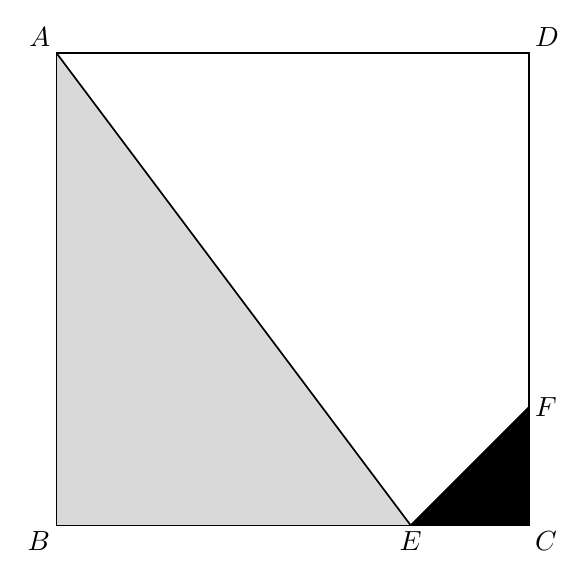
\begin{tikzpicture}[x=1cm,y=1cm,line width=.6pt,
  geometry edge/.style={line width=.6pt},
  geometry label/.style={inner sep=1pt}]
\coordinate (A) at (0,6);
\coordinate (B) at (0,0);
\coordinate (C) at (6,0);
\coordinate (D) at (6,6);
\coordinate (E) at (4.5,0);
\coordinate (F) at (6,1.5);
% 材料区域: 灰三角 ABE(单一材料 2), 黑三角 CFE(单一材料 3)
\fill[gray!30] (A)--(B)--(E)--cycle;
\fill[black] (C)--(F)--(E)--cycle;
% 轮廓与分割线
\draw[geometry edge] (A)--(B)--(C)--(D)--cycle;
\draw[geometry edge] (A)--(E);
\draw[geometry edge] (E)--(F);
% 标签
\node[anchor=south east,inner sep=0pt,xshift=-2pt,yshift=2pt] at (A) {$A$};
\node[anchor=south west,inner sep=0pt,xshift=2pt,yshift=2pt] at (D) {$D$};
\node[anchor=north east,inner sep=0pt,xshift=-2pt,yshift=-2pt] at (B) {$B$};
\node[anchor=north west,inner sep=0pt,xshift=2pt,yshift=-2pt] at (C) {$C$};
\node[anchor=north,inner sep=0pt,yshift=-2pt] at (E) {$E$};
\node[anchor=west,inner sep=0pt,xshift=2pt] at (F) {$F$};
\end{tikzpicture}
